\section{Architekturüberblick}

Die Abbildung 4.1 veranschaulicht die erweiterte REALIS-Architektur zur Realisierung des Feasibility Checks. Basierend auf dem bestehenden REALIS-Komponentendiagramm (siehe Abbildung 2.3) werden neue Komponenten hinzugefügt, um die Feasibility-Check-Funktionalität zu integrieren. Im Diagramm sind dabei aus Gründen der Übersichtlichkeit nur die wichtigsten Erweiterungen dargestellt.

\begin{figure}[!htbp]
    \centering
    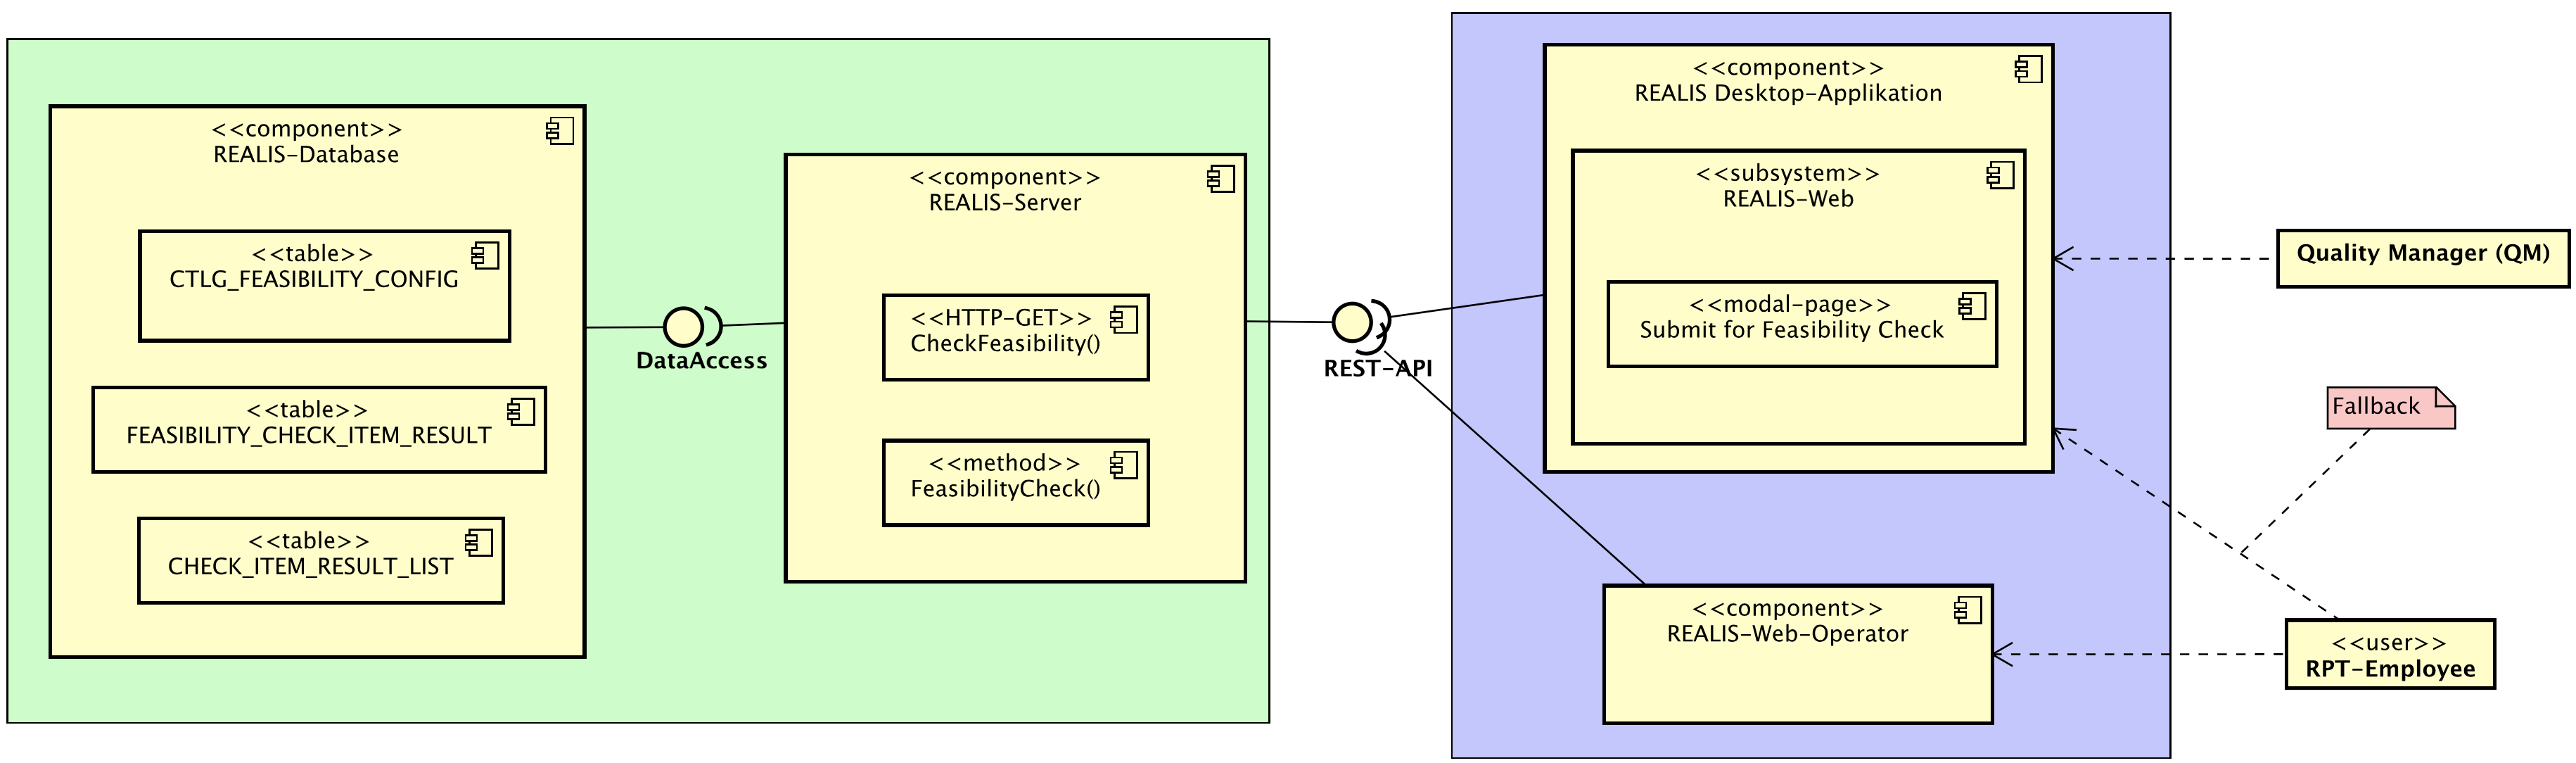
\includegraphics[width=1\textwidth]{bilder/KomponentenDiagramm-REALIS-mitErweiterungen.png}
    \caption{Feasibility Check Architekturdesign-Erweiterung von \gls{REALIS}}
    \label{fig:feasibility-check-komponentendiagramm}
\end{figure}

\todo{maybe add opdataparamtype}

In der \textbf{Datenbank} werden neue Tabellen hinzugefügt, die sowohl zur Konfiguration als auch zur Speicherung der Check-Ergebnisse dienen. Hierzu gehören die Tabellen \texttt{CTLG\_FEASIBILITY\_CONFIG}, \texttt{FEASIBILITY\_CHECK\_ITEM\_RESULT} und \texttt{CHECK\_ITEM\_\-RESULT\_\-LIST}.

Im \textbf{Backend} wird eine HTTP-GET-Methode mit der Bezeichnung \texttt{CheckFeasibility()} implementiert. Diese Methode ruft die Kernlogik der Funktion \texttt{FeasibilityCheck()} auf, die die eigentliche Datenverarbeitung übernimmt, die Ergebnisse in der Datenbank abspeichert und ein einfaches Ergebnis zurückliefert.

Im \textbf{Frontend} wird im \textit{REALIS-Web Subsystem} eine neue Modal-Page \glqq Submit for Feasibility Check\grqq{} integriert, die es Benutzern ermöglicht, den Feasibility Check zu initiieren. Nach der Überprüfung werden die Ergebnisse übersichtlich dargestellt, und zusätzliche Details können bei Bedarf abgerufen werden. 

Durch diese Erweiterungen wird die Feasibility-Check-Funktion nahtlos in die bestehende REALIS-Architektur eingebettet und ermöglicht eine effiziente Interaktion mit den relevanten Benutzern und Systemkomponenten.


